\chapter{Large-distance limit}
\label{chapter_ld}

In this chapter, we investigate the large--distance limit of the Casimir effect
in the plane--sphere geometry. The large--distance limit may also be
interpreted as the small--sphere limit. Thus, large separations of sphere and
plane correspond to high curvatures of the sphere. We will derive an analytical
expression for perfect reflectors which will help us to understand the origin of
the occurence of negative entropies. We will mainly follow the derivation of
Refs. \cite{Durand,ThermalCasimirEffect}.

For large separations of plane and sphere $\mathcal{L} \gg R$ the dominant
contribution to the free energy comes from the dipole moment $\ell = 1$.  The
matrix elements become small and we may approximate the logarithm of the
determinant of the scattering matrix by the trace of the round-trip matrix
\begin{equation}
\log \det \left( \Id - \mathcal{M}^{(m)} \right) \approx - \sum_{P=\PE,\PM} \mathcal{M}_{1,1}^{(m)}(P,P).
\end{equation}
The free energy simplifies to
\begin{equation}
\label{eq:ld_F1}
\mathcal{F}_\text{LD} = - \frac{T}{\pi} {\sum_{n=0}^\infty}^\prime \left[ \frac{1}{2} \mathcal{M}_{1,1}^{(0)}(E,E) + \frac{1}{2} \mathcal{M}_{1,1}^{(0)}(M,M) + \mathcal{M}_{1,1}^{(1)}(E,E) + \mathcal{M}_{1,1}^{(1)}(M,M) \right],
\end{equation}
whereas the first two summands enclosed within the brackets correspond to $m=0$
and are weighted by a factor $1/2$.
The matrix elements $\mathcal{M}^{(m)}_{1,1,p}(P,P)$ contain the prefactor
$\Lambda_{1,1}^{(m)}$, the integrals $A_{1,1,p}^{(m)}$ and $B_{1,1,p}^{(m)}$, and
the Mie coefficients $a_1$ and $b_1$. The Mie coefficients are evaluated at
the argument $\chi = nTR/\mathcal{L}$ and may be approximated by the low frequency limit
\eqref{eq:scattering_ps_mie_approx}
\begin{equation}
\label{eq:ld_mie}
a_1^\text{perf} \simeq - \frac{2}{3} \left(\frac{nTR}{\mathcal{L}}\right)^3, \\
b_1^\text{perf} \simeq   \frac{1}{3} \left(\frac{nTR}{\mathcal{L}}\right)^3.
\end{equation}
The values of $\Lambda$ are given by
\begin{equation}
\label{eq:ld_lambda}
\Lambda_{1,1}^{(0)} = -\frac{3}{2}, \\
\Lambda_{1,1}^{(1)} = -\frac{3}{4},
\end{equation}
and the integrals can easily evaluated analytically
\begin{align}
\nonumber
A_{1,1,p}^{(0)} &= 0, &
A_{1,1,p}^{(1)} &= -r_p \frac{\e^{-2nT}}{2nT}, \\
\label{eq:ld_integrals}
B_{1,1,p}^{(0)} &= r_p \frac{(2nT+1) \, \e^{-2nT}}{4n^3T^3}, &
B_{1,1,p}^{(1)} &= r_p \frac{(2n^2T^2+2nT+1) \, \e^{-2nT}}{4n^3T^3}.
\end{align}
By inserting \eqref{eq:ld_mie}, \eqref{eq:ld_lambda} and
\eqref{eq:ld_integrals} into \eqref{eq:ld_F1} the free energy simplifies to an
infinite sum over the Matsubara frequencies $\xi_n=nT$. The sum can be
evaluated analytically and one obtains an expression for the free energy.
However, in order to understand the origin of negative entropies, we split the
free energy in contributions regarding polarization.

Following an idea of \textsc{G.-L. Ingold}, we calculate the free energy
separately for the contributions
\begin{equation}
\mathcal{F}_\text{LD} = -\frac{T}{\pi} {\sum_{n=0}^\infty}^\prime \left[ {\sum_{m=0}^1}^\prime \sum_{P=\PE,\PM} \sum_{p=\TE,\TM} \mathcal{M}^{(m)}_{1,1,p} \right]
= {\sum_{m=0}^1}^\prime \sum_P \sum_p \mathcal{F}^{(m)}_{P\to p \to P}.
\end{equation}
So, we split up the free energy in eight contributions. The infinite sums can be
evaluated using \eqref{appendix_geom_series}--\eqref{appendix_geom_series_k2}.
For $m=0$ we find
\begin{align}
\mathcal{F}^{(0)}_{\PE\to\TM\to\PE} &= - \frac{T}{16\pi} \left(\frac{R}{\mathcal{L}}\right)^3 \frac{T + \sinh T \cosh T}{\sinh^2 T}, \\
\mathcal{F}^{(0)}_{\PE\to\TE\to\PE} &= 0, \\
\mathcal{F}^{(0)}_{\PM\to\TM\to\PM} &= 0, \\
\mathcal{F}^{(0)}_{\PM\to\TE\to\PM} &= \frac{1}{2} \mathcal{F}^{(0)}_{\PE\to\TM\to\PE},
\end{align}
and for $m=1$
\begin{align}
\mathcal{F}^{(1)}_{\PE\to\TM\to\PE} &= -\frac{T}{16\pi} \left(\frac{R}{\mathcal{L}}\right)^3 \left[\frac{\cosh T}{\sinh T} + \frac{T}{\sinh^2 T} + T^2\frac{\cosh T}{\sinh^3 T}\right], \\
\mathcal{F}^{(1)}_{\PE\to\TE\to\PE} &= -\frac{T^3}{16\pi} \left(\frac{R}{\mathcal{L}}\right)^3 \frac{\cosh T}{\sinh^3 T}, \\
\mathcal{F}^{(1)}_{\PM\to\TM\to\PM} &= \frac{1}{2} \mathcal{F}^{(1)}_{\PE\to\TE\to\PE}, \\
\mathcal{F}^{(1)}_{\PM\to\TE\to\PM} &= \frac{1}{2} \mathcal{F}^{(1)}_{\PE\to\TM\to\PE}.
\end{align}
The polarization $\TM$ on the plane corresponds to the polarization $\PE$ on
the sphere, and $\TE$ on the plane corresponds to $\PM$ on the sphere.

\begin{figure}
  \begin{minipage}[b]{.5\linewidth}
  \centering
  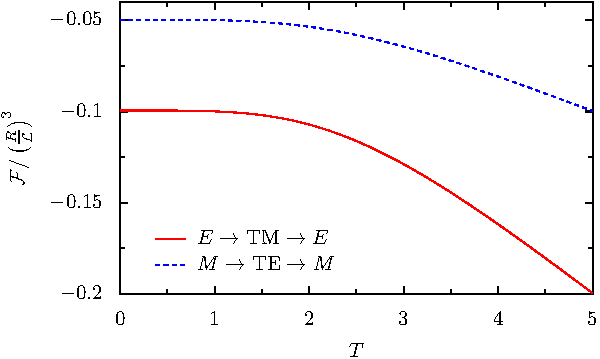
\includegraphics[scale=0.74]{plots/tetm_nochange_ld.pdf}
  \subcaption{no change of polarization}
  \end{minipage}%
  \begin{minipage}[b]{.5\linewidth}
  \centering
  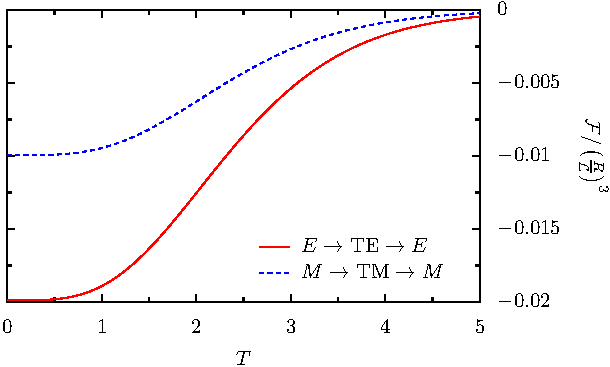
\includegraphics[scale=0.74]{plots/tetm_change_ld.pdf}
  \subcaption{change of polarization}
  \end{minipage}

  \caption{Contributions to the free energy in the large--distance limit for a)
  no change of polarization and b) change of polarization. The solid and dashed
  lines differ by a factor of 2. The contributions in a) decrease and yield
  a positive contribution to the entropy. The contributions in b) increase and
  thus yield a negative contribution to the entropy.}
  \label{fig:ld_F_contrib}
\end{figure}

Adding the contributions of $m=0$ and $m=1$ for the contributions without change of polarization yields
\begin{align}
\label{eq:ld_F_ETME}
\mathcal{F}_{\PE\to\TM\to\PE} &= \frac{-T}{16\pi \, \sinh^3 T} \left(\frac{R}{\mathcal{L}}\right)^3 \left[ 2\cosh T \sinh^2 T + 2 T \sinh T + T^2 \cosh T \right], \\
\label{eq:ld_F_MTEM}
\mathcal{F}_{\PM\to\TE\to\PM} &= \frac{1}{2} \mathcal{F}_{\PE\to\TM\to\PE}.
\end{align}
Both contributions differ by a factor of 2 with $\mathcal{F}_{\PM\to\TE\to\PM}$
being larger in amount. The two contributions to the free energy are depicted in
Fig \ref{fig:ld_F_contrib} a). The contributions to the free energy have zero
slope for $T=0$ and decrease linear for high temperatures. As the slope of the
functions are negative for arbitrary temperatures, the contributions to the
entropy are positive. Moreover, the contributions to the entropy become
constant for high temperatures.

Adding the contributions of $m=0$ and $m=1$ for the contributions with change of polarization yields
\begin{align}
\label{eq:ld_F_ETEE}
\mathcal{F}_{\PE\to\TE\to\PE} &= \frac{-T^3}{16\pi} \left(\frac{R}{\mathcal{L}}\right)^3 \frac{\cosh T}{\sinh^3 T}, \\
\label{eq:ld_F_MTMM}
\mathcal{F}_{\PM\to\TM\to\PM} &= \frac{1}{2} \mathcal{F}_{\PE\to\TE\to\PE}.
\end{align}
Once more both contributions differ by a factor of 2 with
$\mathcal{F}_{\PE\to\TE\to\PE}$ being larger in amount. The two contributions
to the free energy are depicted in Fig \ref{fig:ld_F_contrib} b). Also, the
contributions to the free energy have slope zero for $T=0$. However, the
functions increase and tend to zero for high temperatures. Thus, the
contribution to the entropy is zero for $T=0$, negative for intermediate
temperatures, and tends to zero for high temperatures.

We see that the terms with a change of polarization yield a positive
contribution to the entropy. This means that the change of polarization is the
reason of negative entropies in the plane--sphere geometry. This is certainly
true in the large--distance limit and at least reasonable for arbitrary
separations. For perfect reflectors the entropy is always non-negative in the
plane--plane geometry. For this reason, the entropy in the proximity force
approximation (PFA) is also non-negative. However, we have seen in the last
chapter that for small separations of sphere and plane the PFA becomes
accurate. Therefore the entropy must become non-negative or at least arbitrary
small. As the PFA neglects contributions due to polarization changes, it is
thus at least reasonable that negative entropies are associated with
polarization changes.

\begin{figure}
  \begin{minipage}[b]{.5\linewidth}
  \centering
  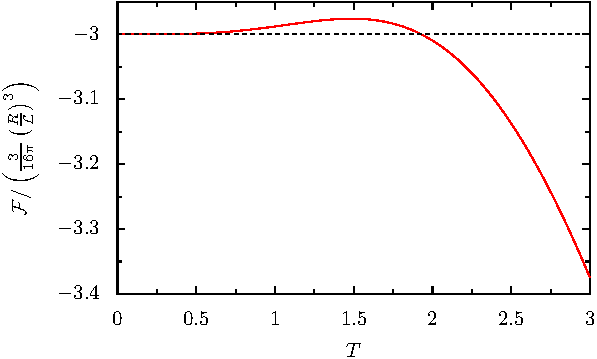
\includegraphics[scale=0.74]{plots/scattering_F_ld.pdf}
  \subcaption{free energy}
  \end{minipage}
  \begin{minipage}[b]{.5\linewidth}
  \centering
  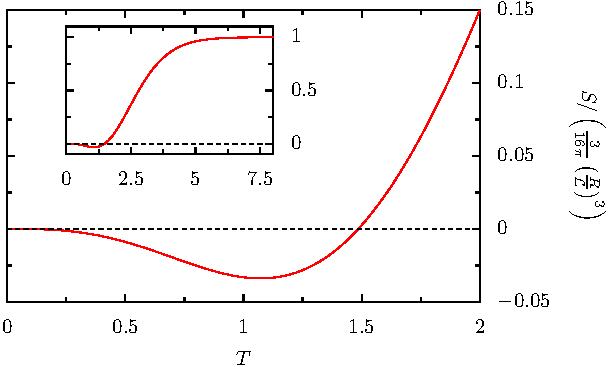
\includegraphics[scale=0.74]{plots/scattering_S_ld.pdf}
  \subcaption{entropy}
  \end{minipage}

  \caption{We plot a) the free energy and b) the entropy dependent on $T$. The free energy increases for small temperatures to a local maximum
  and decreases afterwards, thus yielding negative entropies for $0 < T \lesssim 1.48584$.}
  \label{fig:ld_F}
\end{figure}

By summation of all contributions we obtain for the free energy
\begin{equation}
\label{eq:ld_F_total}
\mathcal{F}_\text{LD} = -\frac{3T}{16\pi} \left(\frac{R}{\mathcal{L}}\right)^3 \frac{T\sinh T + \cosh T\left(T^2+\sinh^2 T\right)}{\sinh^3 T}.
\end{equation}
Interestingly, the effects due to finite temperature and curvature are
separated in this limit. For low temperatures \eqref{eq:ld_F_total} can be
approximated by a Taylor series and we find
\begin{equation}
\label{eq:ld_F_LT}
\mathcal{F}_\text{LD}^\text{LT} \approx -\frac{9}{16\pi} \left(\frac{R}{\mathcal{L}}\right)^3 \left(1 - \frac{T^4}{135} + \frac{4T^6}{945} - \frac{T^8}{945}\right).
\end{equation}
The first finite temperature correction is positive and thus yields a negative
contribution to the entropy. Also, for large separations the factor $R/\mathcal{L}$
decreases and the free energy, the force and the entropy become small.
For high temperatures one obtains
\begin{equation}
\mathcal{F}_\text{LD}^\text{HT} \approx -\frac{3T}{16\pi} \left(\frac{R}{\mathcal{L}}\right)^3.
\end{equation}
In the high temperature limit the free energy descreases proportional to the
temperature, thus yielding a positive and constant entropy.

The free energy and the entropy are depicted in Fig. \ref{fig:ld_F}. For low
temperatures the free energy increases up to a maximum at $T\approx1.48584$ and
decreases for higher temperatures. In the high temperature limit the function
decreases proportional to the temperature. The maximum of the free energy
yields negative entropies in the range $0 \le T \lesssim 1.48584$. As the effect
of negative entropies is caused by a change of polarization, we may assume that
the entropy is always positive for temperatures $T \gtrsim 1.48584$. We will
verify this assumption in chapter \ref{chapter_negative_entropies}.
